\newpage
%\pagestyle{empty}

\begin{minipage}[c]{.25\linewidth}
	
\includegraphics[width=4cm]{images/Logo-LEnsE.png}
\end{minipage} \hfill
\begin{minipage}[c]{.4\linewidth}

\begin{center}
\vspace{0.3cm}
{\Large \textsc{Interféromètre de ZYGO}}

\medskip

\textbf{\Large IHM - \textsc{Masques}}

\end{center}
\end{minipage}\hfill

%%%%%%%%%%%%%%%%%%%%%%%%%%%%%%%%%%
%%%%%%%%%%%%%%%%%%%%%%%%%%%%%%%%%%
\section{Création d'un masque}

La seconde étape avant de pouvoir analyser l'état de surface des optiques est de \textbf{définir un masque sur la zone d'étude}.

Cette étape se fait dans la partie \mbox{\fbox{\textbf{\textsc{Gestion des Masques}}}} de l'application.

\medskip

Cette section permet de :

\begin{itemize}
	\item \textbf{gérer les masques déjà présents} (section \textbf{Affichage des masques}) : suppression, sélection, inversion... 
	\item \textbf{ajouter un nouveau masque} (boutons \textbf{Masque Circulaire}...) d'un certain type
\end{itemize}

\begin{center}
	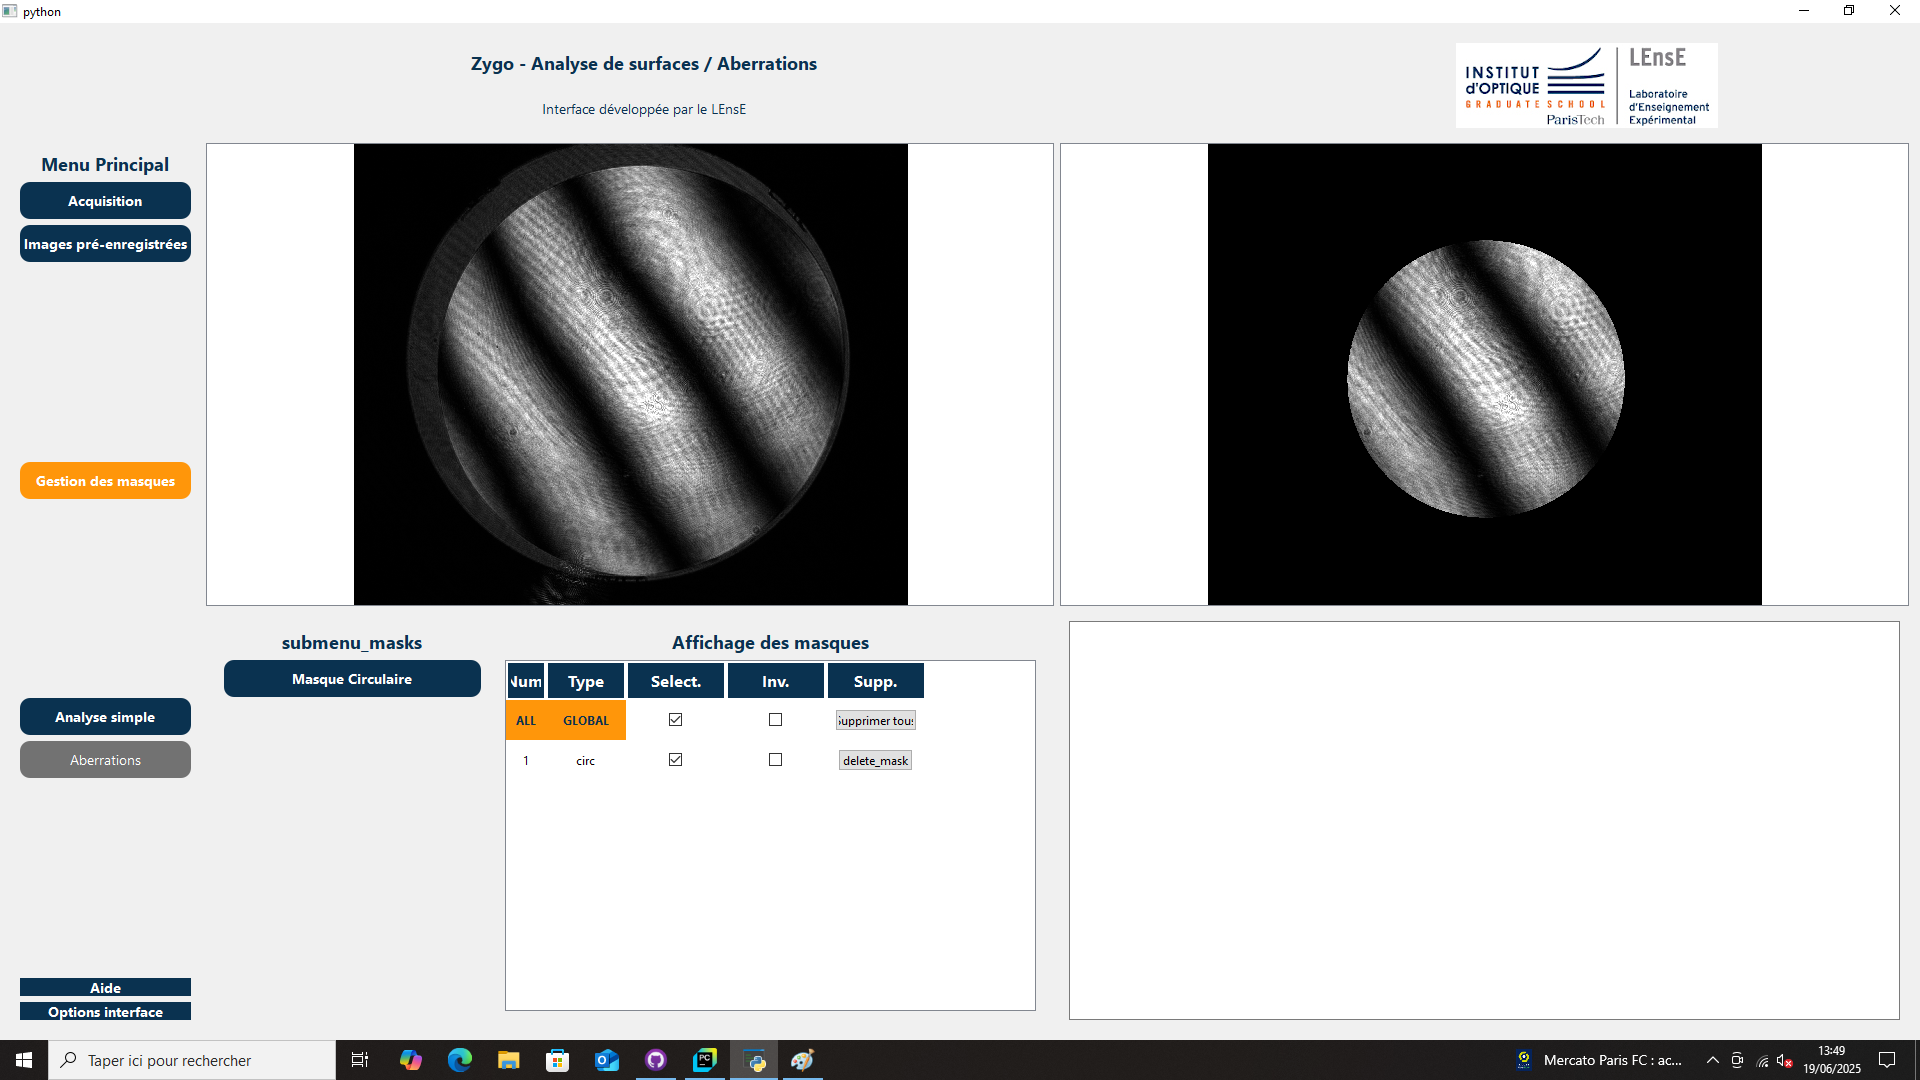
\includegraphics[width=0.9\textwidth]{images/zygo_masques.png}
\end{center}

\subsection{Ajout d'un nouveau masque}

Vous devez cliquer sur l'un des boutons \mbox{\fbox{\textbf{\textsc{Masque ...}}}}, en fonction du type de masque voulu.

\bigskip

Lors de l'ajout d'un masque, une nouvelle fenêtre s'ouvre.

Les \textbf{masques circulaires} nécessitent de choisir \textbf{3 points} dans l'image. Le cercle sera ensuite calculé pour passer par ces trois points.


\begin{tcolorbox}[myboxstyle]
\begin{large}
\begin{center}
Pour l'étude des \textbf{aberrations}, un seul masque est nécessaire. 

Il doit être de type \textbf{circulaire}.
\end{center}
\end{large}
\end{tcolorbox}

